\chapter{Machine Learning}
\label{ch:neural-network}

In this Chapter we will see how machine learning techniques can be
successfully applied to solve financial problems. We will first do a
quick tour on the theory behind neural networks and then we will see 
few examples and practical applications regarding regression and
classification issues.

Beware that this Lecture just scratches the surface of the
machine learning topic which has seen a huge development in the latest
years leading to thousands of applications in many different fields.
    
\section{Neural Networks}\label{neural-networks}

Artificial Neural Networks (ANN or simply NN) are information processing
models that are developed by inspiring from the working principles of
human brain. Their most essential property is the ability of learning
from sample sets.

\subsection{Neurons and Activation Functions}
The basic unit of ANN architecture are neurons which internally may be in
connection with other neurons.

A neuron consists of weights (\(w_i\)) and real numbers (\(x_i\)). All
inputs injected into a neuron are individually weighted, added together
(sometimes it is added also a bias \(w_0\)) and passed into the
activation function which produces the neuron output

\[ \textrm{Inputs} = \sum_{i=1}^{N} x_i w_i +w_0 \rightarrow f(\textrm{Inputs}) = \textrm{Outputs}\]
Figure~\ref{fig:neuron} shows an example.

There are many different types of activation function and two of the simpler are the \emph{step function},
which returns just 0 or 1 according
to the input value, and the \emph{sigmoid} which can be thought
of as the continuous version of the step function, see Fig.~\ref{fig:act_func}.
Other commonly used activation functions are the \emph{Rectified Linear Unit}
(ReLU) and the \emph{hyperbolic tangent} (tanh).

For an deeper discussion of activation functions see this article~\cite{bib:activation_function}.

\begin{figure}[htb]
	\centering
	\subfloat[Model of an artificial neuron.\label{fig:neuron}]{%
		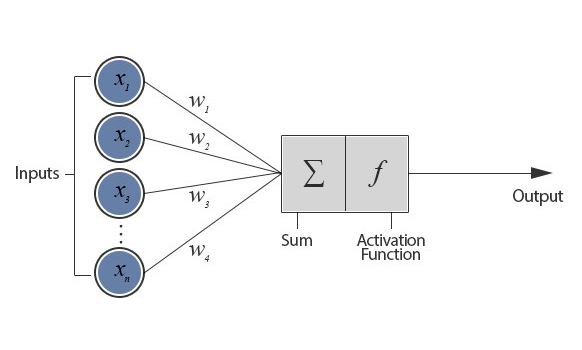
\includegraphics[width=0.6\textwidth]{figures/neuron}
	}
	\subfloat[Examples of sigmoidal and step activation functions.\label{fig:act_func}]{%
		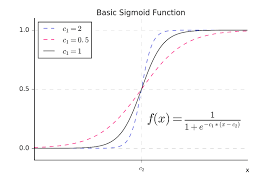
\includegraphics[height=0.30\textwidth]{figures/sigmoid}
	}
	\caption{Basic components of a neuron.}
	\label{fig:sigmoid}
\end{figure}

\subsection{Training of a Neuron}\label{training-of-a-neuron}

When teaching children how to recognize a bus, we just tell them,
showing an example: "This is a bus. That is not a bus." until they
learn the concept of what a bus is. Afterwards, if a child sees new
objects that she hasn't seen before, we could expect her to recognize
correctly whether the new object is a bus or not.

This is exactly the idea behind neuron training. Similarly, inputs from a
\emph{training} set are presented to the neuron one after the other
together with the correct output. During the process neuron weights are modified
so that the neuron response matches the true output.

When an entire pass through all of the input training vectors is
completed (an \emph{epoch}) the neuron has learnt ! (to make it learn better the same
training data is usually processed multiple times)

At this time, when an input vector \(\mathbf{x}\), already in the training
set, is given to the neuron, it will output the correct value. If
\(\mathbf{x}\) is not in the training set, the neuron will respond with
an output close to those corresponding to other training vectors similar to \(\mathbf{x}\).

This kind of training is called \emph{supervised} because we have a set of training data with known targets 
(the true outputs), and we want our model to learn to predict the target from the other variables.

Unfortunately using just a neuron is not too useful since with
such a simple architecture is not possible to solve the interesting problems we would like to face. 
The next step is then to put together more neurons in \emph{layers}.

\subsection{Multilayered Neural Networks}\label{multi-layered-neural-networks}

In a multilayered configuration each neuron from the \emph{input layer} 
is fed up to each node in the
next hidden layer. This kind of connections is repeated for each node down to the output layer. 
We should note that there can be any number of nodes per layer and there
are usually multiple hidden layers to pass through before ultimately
reaching the output layer. Figure~\ref{fig:multilayered_nn} shows a simple
example of such an architecture.

\begin{figure}[htb]
	\centering
	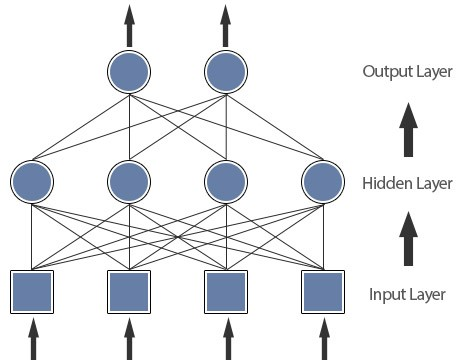
\includegraphics[width=0.6\textwidth]{figures/multilayer.jpeg}
	\caption{A multilayered neural network.}
	\label{fig:multilayered_nn}
\end{figure}

\subsection{Training a Multilayered Neural Network}
\label{training-a-multilayered-neural-network}

The training of a multilayered NN follows these steps:

\begin{itemize}
	\tightlist
	\item
	present a training sample to the neural network (initialized with
	random weights);
	\item
	compute the network output obtained by calculating activation functions of each layer;
	\item
	calculate the error (loss) as the difference between the NN predicted
	and the actual output;
	\item
	having calculated the error, re-adjust the weights of the network such
	that the error decreases;
	\item
	continue the process for all samples several epochs until the
	error is not changing too much (i.e. the process converged).
\end{itemize}
In Figure~\ref{fig:training} an example of training is shown.

\subsubsection{Loss Function}
The NN error is computed by the \emph{loss function}. Different loss functions will give different error estimates for the same prediction, and thus the they have a considerable effect on the performance of any model. Two are the main possible choices

\begin{itemize}
	\tightlist
	\item
	Mean Absolute Error (MAE): the average of the absolute value of the
	differences between the predictions and true values;
	\item
	Root Mean Squared Error (MSE): the square root of the average of the
	squared differences between the predictions and true values.
\end{itemize}

\begin{figure}[htb]
	\centering
	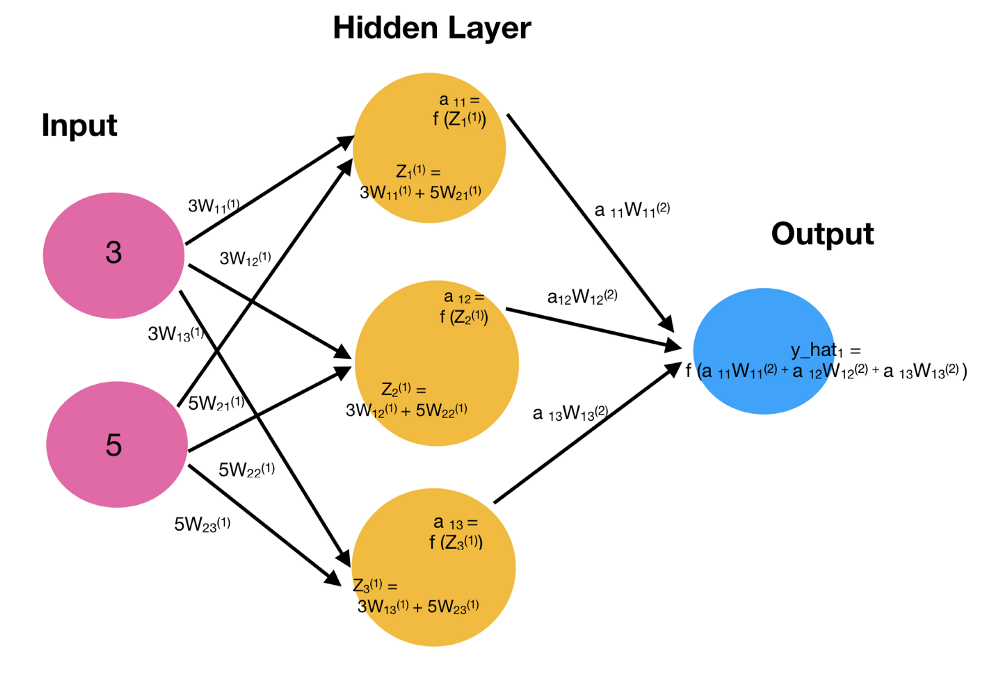
\includegraphics[width=0.9\textwidth]{figures/training_nn}
	\caption{Training example of a multilayered neural network.}
	\label{fig:training}
\end{figure}

The mean absolute error is easily interpreted, as it represents how
far off we are on average from the correct value. The root mean squared 
error instead penalizes larger errors more heavily and is commonly used in
regression tasks. Either metrics may be appropriate depending on the
situation and you can use both for comparison. More information 
about loss function can be found in~\cite{bib:loss_function}.

\subsubsection{Back-propagation}
The loss is a function of the internal parameters of the model
(i.e neuron weights and biases). For an accurate predictions, one needs to
minimize the calculated error and in a neural network, this is done using
\emph{back-propagation}~\cite{bib:backpropagation}.

In this technique the current error is typically "propagated" backwards to previous layers,
where it is used to modify the weights and bias in such a way that the loss tends to be minimized.
The weights are modified with a function called \emph{optimization function}
(we will use \emph{Adam} in the following but there are more).

%\begin{figure}[htb]
%	\centering
%	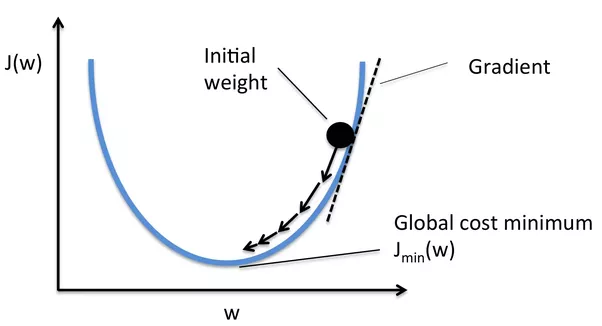
\includegraphics[width=0.7\textwidth]{figures/loss_function}
%	\caption{Optimization of the weights done minimizing the loss function.}
%\end{figure}

\subsection{Overtraining}
A common mistake to avoid during the training is to \emph{overtrain} or \emph{overift} a NN. %Overtraining is  what happens when the NN learns too well the training sample but its performance degrade substantially in an independent testing sample.
Overfitting happens when a model is trained too well on the training data. This means that the model mostly just memorized the training data, and accounts for a large accuracy with the training data but a low accuracy in the testing data. 

To check for overfitting it is required to split the available sample in at least into two parts:
training and testing (e.g.~80\% and 20\%) and to use the former to perform the training and the latter 
to cross-check the performance.
\textbf{Usually performance are measured using the loss function value at the end of the training.}

%Actually you should split the sample in three parts: training, testing and validation. What you would usually do is take the model with the highest validation accuracy and then test the model with the testing set.
%This makes sure that you don’t overfit the model. Using the validation set to choose the best model is a form of data leakage (or “cheating”) to get to pick the result that produced the best test score out of hundreds of them. Data leakage happens when information outside the training data set is used in the model.
%In this case, our testing and validation set are the same, since we have a smaller sample size.

\subsection{Neural Network Design}\label{neural-network-design}

There is no rule to guide developer into the design of a neural network
in terms of number of layers and neurons per layer (the so called hyper-parameters). 

One popular method for hyper-parameter optimization is  the \emph{grid search}. 
With this method a list of possible values for each hyper-parameter is defined, then the model is run multiple times, each time with a different combination of the hyper-parameter values. In the end the hyper-parameter set giving 
the best result is taken. Clearly this is the most thorough way of selecting the neural network architecture 
but it is also the most computationally heavy way to do this.

%The most common strategy is trail and error where you finally pick up the solution giving the best accuracy. In general a larger number of nodes is better to catch highly structured data with a lot of feature although it mayrequire larger training sample to work correctly.
Anyway as a rule of thumb a NN with just one hidden layer with a number
of neurons averaging the inputs and outputs is sufficient in most cases.

In the following we will use more complex networks just for
illustration, but no attempt in optimizing the layout has been done at all.

\subsection{Regression and Classification}\label{regression-and-classification}

The two main categories of problems that can be solved with neural
networks are \emph{classification} and \emph{regression}. Let's see
their characteristics and differences.

\subsubsection{Classification}\label{classification}

Classification is a process of finding a function which helps in dividing
the dataset into classes based on different parameters. 
The task of the classification algorithm is to find the mapping function
to map the input (\(x\)) to the \textbf{discrete} output (\(y\)) or in other words
it tries to find the decision boundary, which can divide the dataset into the
different classes.

A typical example of classification problem is
\emph{email spam detection}. The model is trained on the basis of millions of
emails on different parameters, and whenever it receives a new email, it
identifies whether the email is spam or not. Classification algorithms can also be used in
speech recognition, car plates identification, \ldots

\subsubsection{Regression}\label{regression}

Regression is the process of finding hidden correlations between dependent
variables. It helps in predicting continuous
variables such as market trends, house prices, \ldots

The task of the regression algorithm is to find the mapping function to
map the input variable (\(x\)) to the \textbf{continuous} output
variable (\(y\)), trying to find the best fit which can predict the
output.

As an example suppose we want to do weather forecasting, so for this, we will
use a regression algorithm. The model is trained
on past data, and once the training is completed, it can predict the
weather for future days. In general whenever we are dealing with
function approximations this kind of algorithms can be applied.

\begin{attention}
\subsubsection{Technical Note}\label{technical-note}

Neural network training and testing is performed using two modules:
\texttt{keras}~\cite{bib:keras} (which in turn is based on a Google open source library
called \texttt{tensorflow}~\cite{bib:tensorflow}) and \texttt{scikit-learn}~\cite{bib:scikit} 
which provide many useful utilities.

In order to hide as much as possible the many little details that have to
be set when dealing with NN it has been developed a simple class
(\texttt{FinNN}: Financial NN) which relies on \texttt{keras} anyway 
but should make the whole process easier.
\end{attention}

\section{Function approximation}\label{function-approximation}

As a first practical example let's try to design an ANN which is capable
of learning the functional form underlying a set of data.
The implementation of the neural network starts by importing the necessary modules.

\begin{ipython}
from finnn import FinNN
import numpy as np
\end{ipython}

Then we generate the training sample (i.e. \(x\) input, \(f(x)\) target output
pairs where \(f(x) = x^3 +2\).)
and apply a simple transformation on the sample in order to have all the
inputs and outputs in the \([0, 1]\) range. This is usually done to
provide the NN with \emph{normalized} data, in fact it could be fooled
by very large or very small numbers giving unstable results.

\begin{ipython}
x = np.array([i for i in np.arange(-2, 2, 0.001)])
y = np.array([i**3+2 for i in x])
print("Distribution of original data ", x.min(), x.max(), y.min(), y.max())
trainer = FinNN("ANN")
trainer.setData(x, y, test_size=0.2)
trainer.normalize()
print("The same data after the normalization ", trainer.x.min(),
       trainer.x.max(), trainer.y.min(), trainer.y.max())
\end{ipython}
\begin{ioutput}
Distribution of original data  -2.0 1.9989999999995596 -6.0 9.98800599899472
The same data after the normalization  0.0 1.0 0.0 0.9999999999999999
\end{ioutput}

Next we can define the structure of the neural network itself. 
Here the problem is quite simple so there is no need to use a complicated architecture,
two layers with 15 and 5 neurons respectively and a \texttt{tanh} activation function, 
see Fig,~\ref{fig:ann_1}. The \texttt{inputs} parameter has to be
set to 1 since we have just one single input, the \texttt{x} value.

\begin{ipython}
# design the neural network model
trainer.addInputLayer(inputs=1, neurons=15, activation='tanh')
trainer.addHiddenLayer(neurons=5, activation='tanh')
trainer.addOutputLayer(outputs=1)
# define the loss function (mean squared error)
# and optimization algorithm (Adam)
trainer.compileModel(loss='mse', opt='adam')
# fit the model on the training dataset
trainer.fit(epochs=2000, verbose=1)
\end{ipython}
\begin{ioutput}
Epoch 1/2000
3200/3200 [==============================] - 0s 31us/step - loss: 0.2362
Epoch 2/2000
3200/3200 [==============================] - 0s 6us/step - loss: 0.1498
...
Epoch 1999/2000
3200/3200 [==============================] - 0s 18us/step - loss: 8.7152e-06
Epoch 2000/2000
3200/3200 [==============================] - 0s 17us/step - loss: 5.9604e-06
\end{ioutput}

\begin{figure}[htb]
	\centering
	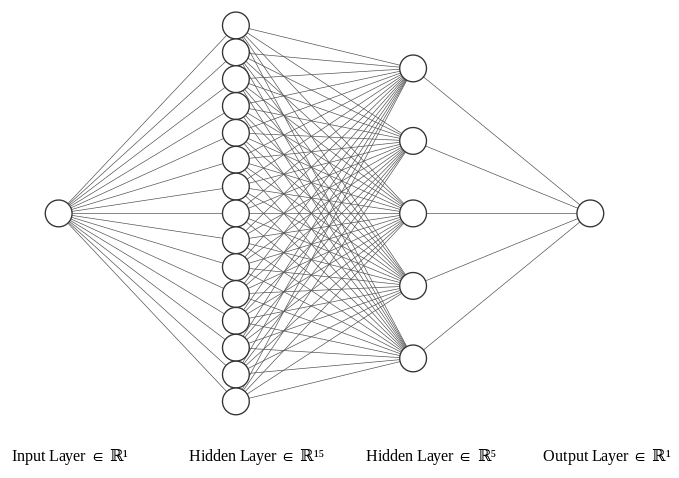
\includegraphics[width=0.9\textwidth]{figures/ann_1.png}
	\caption{Graphical representation of the ANN used to approximate the function $f(x) = x^3 + 2$.}
    \label{fig:ann_1}
\end{figure}

The training output provides a counter with the current epoch number beside the estimated loss
which is evaluated using the loss function chosen in the code.

After the training is completed we can evaluate how good it is by computing the loss with the 
latest update of the network weights. This can be done with the \texttt{evaluate()} method

\begin{ipython}
trainer.evaluate()
\end{ipython}
\begin{ioutput}
3200/3200 [==============================] - 0s 83us/step
Training: 6.1983578859781115e-06
800/800 [==============================] - 0s 52us/step
Test: 6.47684617433697e-06
\end{ioutput}
\noindent
which provides the loss values on training and testing samples.
A \emph{perfect} prediction would have led to \(\textrm{loss}=0\) so the
lower this number the better is our training. 

Clearly the goodness of the model increases with the number of epochs run in the training,
since the NN had more chances to learn the features of the input sample. 
To get an idea of what it is going on in Fig.~\ref{fig:training_vs_epochs} are shown the
actual function we want to approximate and different predictions obtained with the same
NN trained with various number of epochs (i.e. 5, 100, 800, 5000).

\begin{figure}[htb]
	\centering
	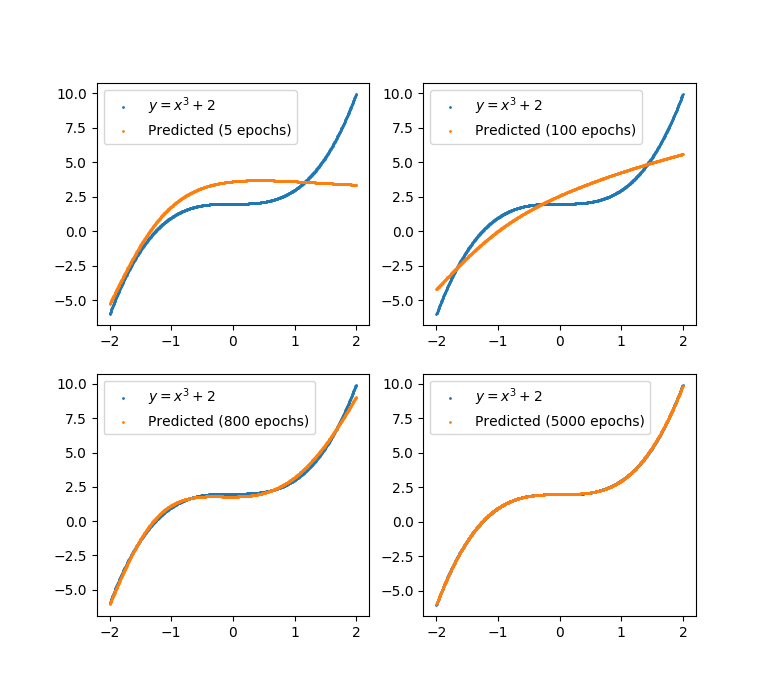
\includegraphics[width=0.9\textwidth]{figures/training_vs_epoch}
	\caption{Prediction of the target $f(x)$ using different number of epochs in the training (5, 100, 800 and 5000) respectively.}
	\label{fig:training_vs_epochs}
\end{figure}

It is clear how the agreement improves with higher number of epochs
which means that the NN has more opportunities to adapt the weights and
reduce the loss to the target values. However, even in the
case of 5000 epochs, zooming in it could be possible to see discrepancies not visible
at the scale of the plot. On the other hand remember that increasing too much the number
of epochs may lead to overfitting. 

To check if this is the case we can compare the loss computed with the training sample
to that on the testing sample. If the two numbers are comparable the NN is
ok, otherwise if the loss on the training is much smaller than the testing we
had overfitting.

In our example since the two numbers are in good agreement we can be confident that 
there hasn't been overtraining.
In case one need more accuracy and has already incremented too much the number of epochs
could either increase the size of the training sample or change the NN architecture.

\subsection{Black-Scholes call
options}\label{black-scholes-call-options}

The first financial machine learning application concerns the pricing of european
call options: essentially we will create a neural network capable of
approximate the famous Black-Scholes pricing formula

\begin{equation} 
	P_\textrm{call} = F_\textrm{BS}(K, r, \sigma, \mathrm{ttm})
\end{equation}

Like before the first step consists of generating the training sample this time made
of a grid of volatility ($\sigma$)-rate ($r$) pairs (for simplicity we
are going to set moneyness ($K$) and time to maturity (ttm) to 1). The target values
are the price of a call, computed with the corresponding inputs, using the BS function in \texttt{finmarkets.py}.

\begin{ipython}
from finmarkets import call

data = []
rates = np.arange(0.01, 0.11, 0.001)
sigmas = np.arange(0.1, 0.6, 0.005)

for r in rates:
for sigma in sigmas:
call_price = call(1, r, sigma, 1)
data.append([r, sigma, call_price])

# we transform the list to a numpy array just because
# an array is more convenient to use later
data = np.array(data)
\end{ipython}

Since it takes some time to generate data samples, it is always
advisable to save them in a file since we may need to load it many times
during the NN development. This can be done with \texttt{pandas}

\begin{ipython}
import pandas as pd

df = pd.DataFrame()
df['rate'] = data[:, 0]
df['vol'] = data[:, 1]
df['price'] = data[:, 2]
df.to_csv("bs_training_sample.csv")

print (df.describe())
\end{ipython}
\begin{ioutput}
               rate           vol         price
count  10000.000000  10000.000000  10000.000000
mean       0.059500      0.347500      0.165274
std        0.028868      0.144338      0.055387
min        0.010000      0.100000      0.044852
25%        0.034750      0.223750      0.119389
50%        0.059500      0.347500      0.165476
75%        0.084250      0.471250      0.212097
max        0.109000      0.595000      0.277071
\end{ioutput}

Following the previous example we will use the \texttt{FinNN}
class to develop the NN and also we will \emph{normalize} data to get
better results. \textbf{Beware that this time we have TWO input
parameters (rate and volatility)}. See Figure~\ref{fig:ann_2} for
a graphical representation of the designed ANN.

\begin{figure}[htb]
	\centering
	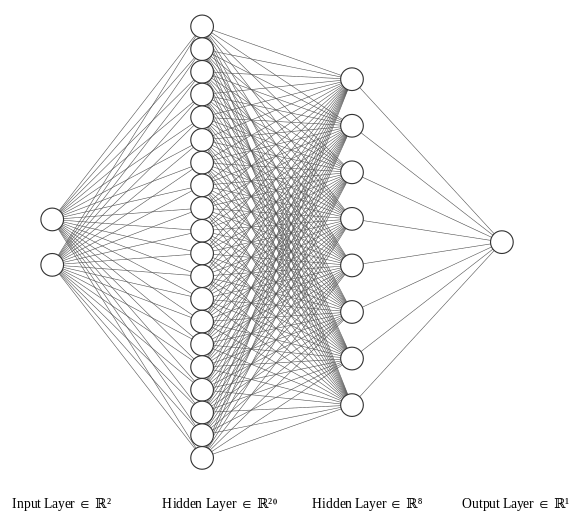
\includegraphics[width=0.9\textwidth]{figures/ann_2.png}
	\caption{Graphical representation of the ANN used to approximate the Black and Scholes oprion price function.}
	\label{fig:ann_2}
\end{figure}

\begin{ipython}
data = pd.read_csv("bs_training_sample.csv")
x = data.iloc[:, 1:3].values
y = data.iloc[:, 3].values

trainer = FinNN("ANN")
trainer.setData(x, y, test_size=0.20)
trainer.normalize()
trainer.addInputLayer(inputs=2, neurons=20, activation='relu')
trainer.addHiddenLayer(neurons=8, activation='relu')
trainer.addOutputLayer(outputs=1)

trainer.compileModel(loss='mse', opt='adam')
trainer.fit(epochs=3000, batch_size=500, verbose=1)
\end{ipython}
\begin{ioutput}
Epoch 1/3000
8000/8000 [==============================] - 0s 16us/step - loss: 0.3216
Epoch 2/3000
8000/8000 [==============================] - 0s 4us/step - loss: 0.2620
...
Epoch 2999/3000
8000/8000 [==============================] - 0s 4us/step - loss: 3.7983e-07
Epoch 3000/3000
8000/8000 [==============================] - 0s 3us/step - loss: 3.6476e-07
\end{ioutput}
\begin{ipython}
trainer.evaluate()

# when the training takes some time it is useful
# to save the model weights in a file to use it later on
trainer.saveModel('black_scholes')
\end{ipython}
\begin{ioutput}
8000/8000 [==============================] - 0s 52us/step
Training: 5.567638540924235e-07
2000/2000 [==============================] - 0s 44us/step
Test: 5.582978365055169e-07
\end{ioutput}

As you can see the training and testing samples give roughly the same MSE value so we are reasonably sure that there hasn't been \emph{overfitting}.
After the training is completed we can evaluate graphically how good it is, see Fig.~\ref{fig:vol_rate}. 

\begin{figure}[htb]
	\centering
	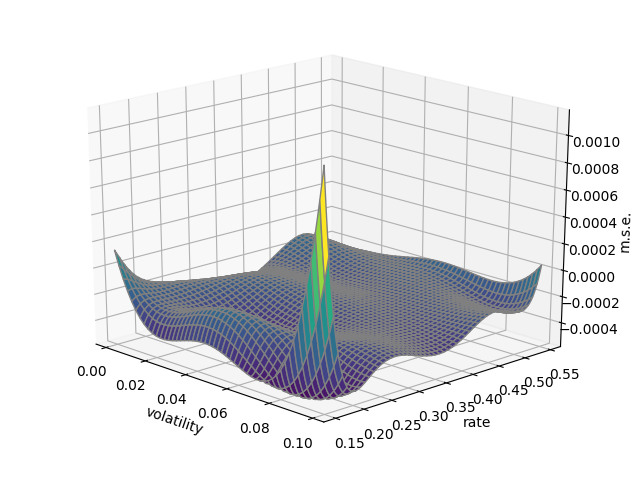
\includegraphics[width=0.7\textwidth]{figures/vol_rate}
	\caption{Mean squared error as a function of volatility and rate for our Black-Scholes function prediction.}
	\label{fig:vol_rate}
\end{figure}

In general to judge if the level of accuracy of your model is enough for your needs you have to 
compare the error in a typical use case (remember that if you are using the MSE metric you need to use
\(\sqrt{\mathrm{MSE}}\) as the \emph{real} error).

In this example we know that our prices go from 0.04 to 0.28 and the
final accuracy is 0.0008. So in the
worst case we are able to price our call as \(0.04 \pm 0.0008\), so a 2\% relative 
error in estimating the call price which is not bad for our study but may be far from ideal for 
an investment.

Let's compare the prediction in a practical case; say we
want to know the price of a call (with moneyness 1 and time to maturity
1 year) when the risk-free rate is 0.015 and the volatility 0.234:

\begin{ipython}
import numpy as np
from finmarkets import call

# here we load the trained model
trainer.loadModel('black_scholes')

# this is our input vector
rv = np.array([[0.015, 0.234]])
# here we compare the predection with the BS call price

print ('{} => {:.4f} (expected {:.4f})'.format(rv.tolist(),
                                               trainer.predict(rv)[0][0],
                                               call(1, rv[0][0], rv[0][1], 1)))
\end{ipython}
\begin{ioutput}
[[0.015, 0.234]] => 0.1001 (expected 0.1001)
\end{ioutput}

It is very import to remember that a \textbf{NN cannot extrapolate}.
Indeed if you try to predict the price of a call from rate and
volatility outside the training \emph{phase space} (i.e. with values that
aren't in the intervals used in the training), say \(r = 0.22\) and
\(\sigma = 0.01\)\ldots{}

\begin{ipython}
# this is our input vector
rv = np.array([[0.22, 0.01]])

# here we compare the predection with the BS call price

print ('{} => {:.4f} (expected {:.4f})'.format(rv.tolist(),
                                        trainer.predict(rv)[0][0],
                                        call(1, rv[0][0], rv[0][1], 1)))
\end{ipython}
\begin{ioutput}
[[0.22, 0.01]] => 0.1628 (expected 0.1975)
\end{ioutput}

\subsection{Model Calibration}\label{model-calibration}

The function approximation capabilities of a neural network can serve
other scopes rather than predicting the function values themselves. Another very useful
application is \emph{model calibration} which consists of
deriving parameters of a model directly from market values. This is
especially convenient to estimate parameters which are
otherwise complicated to compute (e.g. there is no analytic formula to get these parameters).

For simplicity let's keep working with the Black-Scholes formula.
Assume we need to estimate the \emph{implied volatility} of a security in real time. 
The idea is to train a NN similar to the previous one, where the input now is a list of price,
moneyness, rate and time to maturity and the target output is the
volatility. Basically we are trying to approximate an inversion of the the BS formula which
return the underlying volatility

\begin{equation} 
	\sigma = F^{-1}_\textrm{BS}(P_\textrm{call}, K, r, \mathrm{ttm})
\end{equation}

In our examples we have never made any assumption on the functional form of the relation we wanted to approximate
but we have just relied on the capability of NN to learn from the training dataset. 

So calibration in this case means to determine a parameter of the Black-Scholes formula (the volatility) from 
the market prices of the options and their characteristics.

\begin{attention}
\subsubsection{Historical vs. Implied Volatility}
\label{historical-vs.-implied-volatility}

Historical volatility is the realized volatility of the underlying asset over a previous time period. It is determined by measuring the standard deviation of the underlying asset from the mean during that time period.

In contrast to historical volatility, which looks at actual stock prices in the past, \emph{implied volatility} looks toward the future. Implied volatility is often interpreted as the market's expectation for the future volatility of a stock and can be derived from the price of an option (e.g. from the Black and Scholes formula).
Specifically, it is the expected future volatility of the stock that is implied by the price of the stock's options.

The implied volatility of an asset can also be compared with what it was in the past. If a stock has an implied volatility of 40\% compared with a 20\% implied volatility, say, a month ago, the market now considers the stock to be more volatile particularly going forward.

Volatility shifts as markets go through different regimes. Thus, historical volatility may not be an accurate measure of future volatility. Implied volatility takes into account all information used by market participants to 
determine prices in the options market, instead of just past prices.

%In general, if implied volatility is higher than historical volatility it gives some indication that option prices may be high. If implied volatility is below historical volatility, this may mean option prices are discounted and may be “cheap.”
\end{attention}

To reuse the training sample created before (again we
are going to set \(\mathrm{ttm}=1\) and \(K=1\)) now we need to set the input as pairs of rate-price and the
output is the target volatility.

\begin{ipython}
data = pd.read_csv("bs_training_sample.csv")
df = pd.concat([data.iloc[:, 1:2], data.iloc[:, 3:4]], 1))

x = df.values
y = data.iloc[:, 1].values

trainer = FinNN("ANN")
trainer.setData(x, y, test_size=0.20)
trainer.normalize()
trainer.addInputLayer(inputs=2, neurons=20, activation='relu')
trainer.addHiddenLayer(neurons=8, activation='relu')
trainer.addOutputLayer(outputs=1)

trainer.compileModel(loss='mse', opt='adam')
trainer.fit(epochs=2000, verbose=1)

trainer.evaluate()
trainer.saveModel("calibration")
\end{ipython}
\begin{ioutput}
Epoch 1/2000
8000/8000 [==============================] - 0s 14us/step - loss: 0.1339
Epoch 2/2000
8000/8000 [==============================] - 0s 4us/step - loss: 0.1052
...
Epoch 1999/2000
8000/8000 [==============================] - 0s 10us/step - loss: 1.9519e-06
Epoch 2000/2000
8000/8000 [==============================] - 0s 10us/step - loss: 1.9708e-06

8000/8000 [==============================] - 0s 61us/step
Training: 2.0318084630162047e-06
2000/2000 [==============================] - 0s 48us/step
Test: 1.8580968553578714e-06
\end{ioutput}

Provided our training includes the correct range of market prices of our
call we can quickly and easily estimate the implied volatility. For
example if the risk-free rate is 2\% and the current price is 0.15
(remember that we are using the BS formula in terms of moneyness)

\begin{ipython}
trainer.loadModel('calibration')
rv = np.array([[0.02, 0.15]])

print ('{} => {:.4f} (expected call price {:.4f})'.format(rv.tolist(),
                                                   trainer.predict(rv)[0][0],
                                                   call(1, 0.02, 
                                                   trainer.predict(rv)[0][0], 1))
\end{ipython}
\begin{ioutput}
[[0.02, 0.15]] => 0.3565 (expected call price 0.1502)
\end{ioutput}
\noindent
The expected call price (0.1502) derived using the implied volatility is in excellent agreement we the "market price" (0.15).

\section{Neural net to recognize handwritten digits}
\label{neural-net-to-recognize-handwritten-digits}

We don't usually appreciate how tough a problem our visual system solve every time we look at something.
Maybe it is enough to consider that it involves 5 visual cortices containing 140 million neurons each. 
Anyway the difficulties of visual pattern recognition become apparent if you attempt to write a computer
program to recognize digits like those in Fig.~\ref{fig:mnist}.

\begin{figure}[htb]
	\centering
	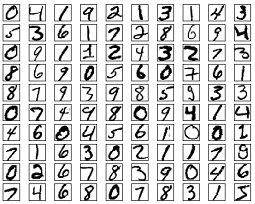
\includegraphics[width=0.5\textwidth]{figures/mnist_100_digits}
	\caption{MNIST sample of handwritten digits.}
	\label{fig:mnist}
\end{figure}

Simple intuition about how we recognize shapes (e.g. a 9 has a loop at
the top, and a vertical stroke in the bottom right) turns out to be not
so simple to express algorithmically. When you try to make such rules
precise, you quickly get lost in a morass of exceptions and caveats and
special cases so that it seems hopeless.

Neural networks approach the problem in a different way. The idea is to
take a large number of handwritten digits and then develop a system
which can learn from those.

By increasing the number of training examples, the network can learn
more and more about handwriting, and so improve its accuracy. So while
it has been shown just 100 training digits above, we could certainly
build a better handwriting recognizer by using thousands or even
millions or billions of training examples (\textbf{as we have seen above
neural nets are not capable of extrapolating results, hence in general it won't
recognize a digit written in some strange way not included in the
training sample !!!}).

In this example we will use the sample provided with the \texttt{mnist} module.
Our program will be based on a slightly different kind of neural network
than before, one type specifically designed for image/pattern
recognition, the Convolutional Neural Network (CNN). We won't go into
the details of its implementation since it is outside the scope of these
Lectures but it works essentially by applying on top of an image 
series of filters (\emph{convolutional layers}) that works as edge
detectors. With them it classifies the images according to their
relevant features.

Convolutional layers prove to be very effective, and stacking them allows to
learn low-level features (e.g. lines) and high-order, or more abstract,
features, like shapes or specific objects, see Fig.~\ref{fig:conv_filters}.

\begin{figure}[htb]
	\centering
	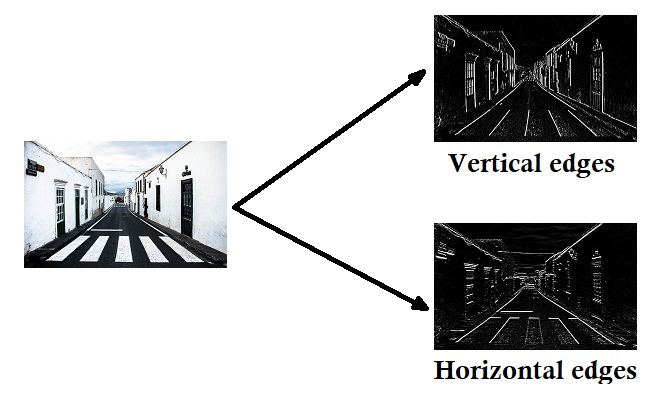
\includegraphics[width=1.\textwidth]{figures/edges.jpg}
	\caption{Edge detected by different layers of a convolutional neural network.}
        \label{fig:conv_fitlers}
\end{figure}

Another important difference with respect to the previous examples is
that in this case we are going to solve a classification problem
(contrary to before when we were trying to regress a sample). Indeed our
NN output won't be a single number but rather a list containing the
probabilities that an image belong to each class.

\begin{ipython}
import numpy as np, mnist
from finnn import FinNN

# the actual
train_images = mnist.train_images()
# the target
train_labels = mnist.train_labels() # (it is a 0, 1, 2...)

# no test_size option means not split the sample
# in training and testing sets
# (MNIST has already dont it for us)

trainer = FinNN("CNN2D")
trainer.setData(train_images, train_labels)
\end{ipython}
\noindent
Next we define the CNN architecture, see Fig.~\ref{fig:cnn2d}.

\begin{ipython}
# define our convolutional NN
# we decide to apply 8 filters to the images
# each with 3x3 pixels size
# the input images have 28x28 pixels size instead
trainer.addConv2DLayer(filters=8, filter_size=3, input_shape=(28, 28, 1))
trainer.addMaxPooling2D(2)
trainer.addFlatten()
trainer.addCNNOutputLayer(outputs=10)

trainer.compileModel(loss='categorical_crossentropy', opt='adam')
trainer.fit(epochs=5, verbose=1)
trainer.saveModel('digit_training')
\end{ipython}
\begin{ioutput}
Epoch 1/5
59999/59999 [==============================] - 13s 210us/step - loss: 2.1711
Epoch 2/5
59999/59999 [==============================] - 12s 201us/step - loss: 0.3964
Epoch 3/5
59999/59999 [==============================] - 12s 199us/step - loss: 0.2655
Epoch 4/5
59999/59999 [==============================] - 12s 198us/step - loss: 0.2244
Epoch 5/5
59999/59999 [==============================] - 12s 196us/step - loss: 0.1910
\end{ioutput}

\begin{figure}[htb]
	\centering
	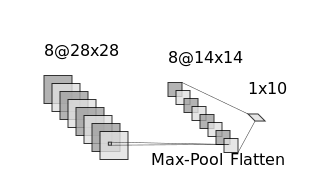
\includegraphics[width=0.9\textwidth]{figures/cnn_2d.png}
	\caption{Graphical representation of the CNN developed to recognize handwritten digits.}
        \label{fig:cnn2d}
\end{figure}

\begin{attention}
\subsubsection{Pooling}

Looking closely to the convolutional neural network implementation we can notice new kind of 
layers never used before, in particular the \texttt{MaxPooling2} layer.

Convolutional layers in a CNN systematically
apply filters to input images in order to create feature maps
that summarize the main characteristics of the sample.

A limitation of the feature map output of convolutional layers is that
they record the precise position of features in the input. This means
that small movements in the position of the feature in the input image
will result in a different feature map. This can happen with
cropping, rotation, shifting, and other minor changes to the input
image.

Imagine a program that look for car plates in pictures taken by a speed
radar, cars won't be in the same position in the frame so there may be
differences in the classification of similar (but not equal) pictures.

A common approach to address this problem is called \emph{down sampling}. 
This is where a lower resolution version of
an input signal (e.g. the picture) is created that still contains the
large or important structural elements, without the fine detail that may
not be as useful to the task.

Down sampling can be achieved using a pooling layer.

Pooling involves selecting a pooling operation, much like a filter to be
applied to feature maps. The size of the pooling operation is
smaller than the size of the feature map; specifically, it is almost
always 2×2 pixels. This means that the pooling layer will always reduce
the size of each feature map by a factor of 2, e.g. each dimension is
halved. For example, a pooling layer applied to a feature map of 6×6 (36
pixels) will result in an output pooled feature map of 3×3 (9 pixels).

The most common pooling operation are:
\begin{itemize}
	\tightlist
	\item Average Pooling: calculate the
	average value for each patch on the feature map;
	\item Maximum Pooling (or Max Pooling): calculate the maximum value for each patch of the feature
	map.
\end{itemize}
\end{attention}

Now let's try to see how well our NN predicts \texttt{mnist} testing
digits.

\begin{ipython}
trainer.loadModel('digit_training')
# testing with mnist test sample
test_images = mnist.test_images()
test_labels = mnist.test_labels()
trainer.setTestData(test_images, test_labels)
predictions = trainer.predict(trainer.x_test[:10])

print ("Tesing on MNIST digits...")
print("Predicted: ", np.argmax(predictions, axis=1))
print("Truth:", test_labels[:10])
print("highest prob.:", ["{:.6f}".format(p[np.argmax(p)]) for p in predictions])
\end{ipython}
\begin{ioutput}
Tesing on MNIST digits...
Predicted:  [7 2 1 0 4 1 4 4 5 9]
Truth: [7 2 1 0 4 1 4 9 5 9]
highest prob.: ['0.999900', '1.000000', '0.999977', '1.000000', '0.999993',
'0.999596', '0.970003', '0.900420', '0.840930', '0.999472']
\end{ioutput}

Since the last but one digit has lower probability let's check the
returned list to see which other number have non-zero probability.

\begin{ipython}
for i, p in enumerate(predictions[8])])
    print("9th digit:", ["dig {}: {:.6f}".format(i, p)
\end{ipython}
\begin{ioutput}
9th digit: ['dig 0: 0.000080', 'dig 1: 0.000000', 'dig 2: 0.000091', 'dig 3:
0.000000', 'dig 4: 0.000000', 'dig 5: 0.840930', 'dig 6: 0.158898', 'dig 7:
0.000000', 'dig 8: 0.000001', 'dig 9: 0.000000']
\end{ioutput}

So the second ranked digit is a 6 (which can be confused with a five if
the lower loop is almost closed).

To see how well our NN behaves with different kind of digits we will try
to check how it works with my calligraphy.
Before passing the image to the NN it has to be resized and this is done
with an ad-hoc function, \texttt{transform\_image}, which is in the
\href{https://raw.githubusercontent.com/matteosan1/finance_course/develop/libro/input_files/digit_converter.py}{\texttt{digit\_converter.py}} module.

\begin{ipython}
from digit_converter import transform_image

filenames = ['four.png', 'five.png']
for f in filenames:
    test_images = np.array(transform_image(f))
test_images = np.expand_dims(test_images, axis=3)
predict = trainer.predict(test_images)

print ("Tesing on custom digits...")
print ("Predicted: ", np.argmax(predict, axis=1))
print("%:", ["{:.3f}".format(p[np.argmax(p)]) for p in predict])
print(["{:.2f}".format(p) for p in predict[0]])
\end{ipython}
\begin{ioutput}
Tesing on custom digits...
Predicted:  [4]
%: ['0.802']
['0.00', '0.00', '0.00', '0.00', '0.80', '0.00', '0.00', '0.20', '0.00', '0.00']

Tesing on custom digits...
Predicted:  [5]
%: ['0.981']
['0.00', '0.00', '0.00', '0.01', '0.00', '0.98', '0.00', '0.01', '0.00', '0.00']
\end{ioutput}
The handwritten images used in this test are shown in Fig.~\ref{fig:test_images}.

\begin{figure}[htb]
	\centering
	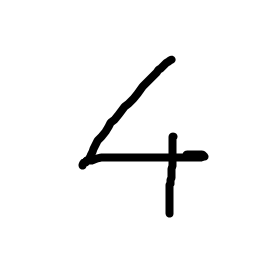
\includegraphics[width=0.2\textwidth]{figures/four.png}
	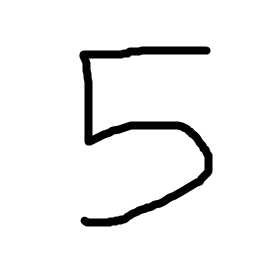
\includegraphics[width=0.2\textwidth]{figures/five.png}
	\caption{Test handwritten digits used in the example.}
	\label{fig:test_images}
\end{figure}

\subsection{Model Calibration cont.}\label{model-calibration-cont.}

When the parameters of the model we want to calibrate can be expressed
as a function of three variables we can implement a convolutional neural network to work with special images representing our model.

Consider again the Black and Scholes formula for the call options.
Assume you need to calibrate the rate \(r\) and the volatity \(\sigma\)
at the same time.% A convolutional neural network can be trained using
%special images which represents \(\mathrm{ttm}, K\) and
%\(P_\textrm{call}\).

A black-white image indeed can be interpreted as a map where each pixel coordinates
is a pair (\(\mathrm{ttm}, K)\) and the pixel color, an integer between
0 (black) and 255 (white), represents \(P_\textrm{call}\). As in the
previous examples the neural network was classifying the pictures into
digits, now it will assign them to classes identified by \(r, \sigma\)
pairs.

The creation of the training sample is a little more complicated now.
For convenience we will use also a new format to save data image,
\texttt{numpy}. This will be done through the corresponding module
simply using the functions \texttt{save} and \texttt{load} to store and
retrieve data. The module \texttt{PIL} (pillow) is instead used to
visualize the images.

First we make the targets.

\begin{ipython}
import numpy as np
from finmarkets import call

labels = []
rates = np.arange(0.01, 0.11, 0.001)
vols = np.arange(0.1, 0.6, 0.005)
for i in range(len(vols)):
    for j in range(len(rates)):
        labels.append((vols[i], rates[j]))
\end{ipython}
\noindent
Then we can create the images.

\begin{ipython}
k = np.arange(0.8, 1.2, (1.2-0.8)/20)
ttm = np.arange(1, 5, 4/20)

# for each r, sigma pair
# generate a matrix of prices
maximum = 0
minimum = np.inf
prices = []
for v in vols:
    for r in rates:
        price = np.zeros(shape=(20, 20))
        for ik, kv in enumerate(k):
            for it, t in enumerate(ttm):
                price[ik, it] = call(kv, r, v, t)
                prices.append(price)
                # max and min are saved to
                # normalize our matrices
                new_max = np.max(price)
                new_min = np.min(price)
                if new_max > maximum:
                    maximum = new_max
                if new_min < minimum:
                    minimum = new_min
for ip, p in enumerate(prices):
    prices[ip] = np.interp(p, (minimum, maximum), (0, 1))
np.save("2d", prices)
\end{ipython}
\noindent
An example of the 20x20 images that have been created is shown in Fig.~\ref{fig:test_images_calib}.

\begin{figure}[htb]
\centering

\includegraphics[width=0.45\textwidth]{figures/2d_training_images}
	\caption{Example of images used to encode calibration information.}
\label{fig:test_images_calib}
\end{figure}
\noindent
Then the training is similar to what has been done for the handwritten
digits.

\begin{ipython}
import numpy as np
from finnn import FinNN

labels = np.load("2d_labels.npy")
images = np.load("2d.npy")

trainer = FinNN("CNN2D")
trainer.setData(images, labels, test_size=0.2)
trainer.addConv2DLayer(filters=8, filter_size=10,
input_shape=(20, 20, 1), activation='relu')
trainer.addFlatten()
trainer.addHiddenLayer(neurons=10, activation='relu')
trainer.addOutputLayer(outputs=2, activation='relu')

trainer.compileModel(loss='mse', opt='adam')
trainer.fit(epochs=500, verbose=1)
trainer.saveModel("2d")
trainer.evaluate()
\end{ipython}
\begin{ioutput}
Epoch 1/500
8000/8000 [==============================] - 1s 156us/step - loss: 0.0018
Epoch 2/500
8000/8000 [==============================] - 1s 142us/step - loss: 6.2310e-04
...
Epoch 499/500
8000/8000 [==============================] - 2s 194us/step - loss: 1.4921e-06
Epoch 500/500
8000/8000 [==============================] - 2s 193us/step - loss: 1.4413e-06

8000/8000 [==============================] - 1s 65us/step
Training: 1.1013161047230825e-05
2000/2000 [==============================] - 0s 70us/step
Test: 1.116331470257137e-05
\end{ioutput}

At this point the test of the trained CNN consists of presenting the prices of call
referring to the same underlying in the pictorial form shown before and
in response it will give the risk-free rate and the underlying volatility.

\begin{ipython}
for i in range(5):
    print (trainer.predict(trainer.x_test[i:i+1]))
\end{ipython}
\begin{ioutput}
[[0.3825101  0.09229672]]
[[0.4056808  0.02232919]]
[[0.47402808 0.05630913]]
[[0.2851617  0.05214534]]
[[0.17245176 0.08815573]]
\end{ioutput}

\section{Technical Analysis}\label{technical-analysis}

In finance \emph{technical analysis} is a security analysis discipline
for forecasting the direction of prices through the study of past market
data, primarily price and volume. Essentially the analyst looks for
particular patterns in the price time series that are believed to
develop in a predictable way to take profit of it, Fig.~\ref{fig:tech_ana} shows two
of such patterns.

\begin{figure}[htb]
	\centering
	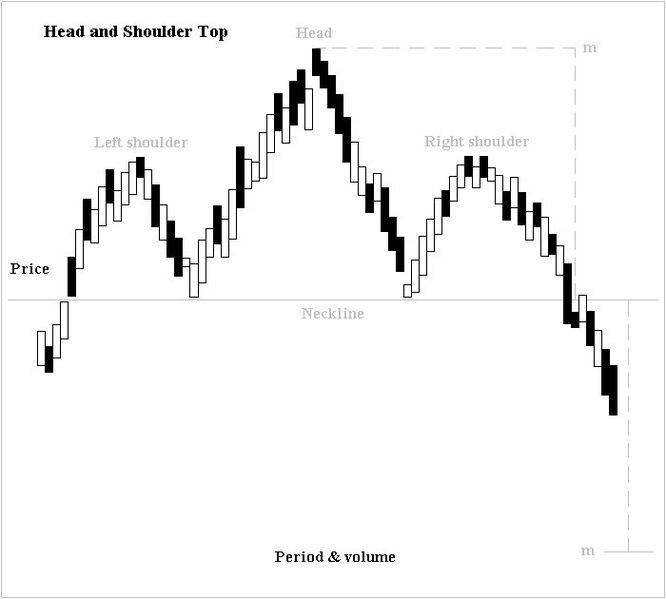
\includegraphics[width=0.4\linewidth]{figures/H_and_s_top_new.jpg}\qquad
	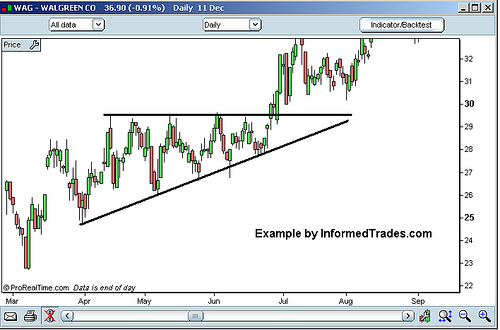
\includegraphics[width=0.4\linewidth]{figures/Triangle-ascending.jpg}
	\caption{Examples of patterns in real time series, head and shoulder (left), triangle (right).}
        \label{fig:tech_ana}
\end{figure}

As you may imagine we will try to develop a CNN capable of classifying features 
in time series to be used in technical analysis (this is much faster than having somebody looking at
thousands of time series by eye).

The training sample is made of 21600 time series
(1/3 with head and shoulder patter, 1/3 with triangle pattern and 1/3
with no pattern), see Fig~\ref{fig:patterns}.
\emph{To make the training easier the features are quite exaggerated.}

\begin{figure}[htbp]
	\centering
	\subfloat[No pattern.\label{}]{%
		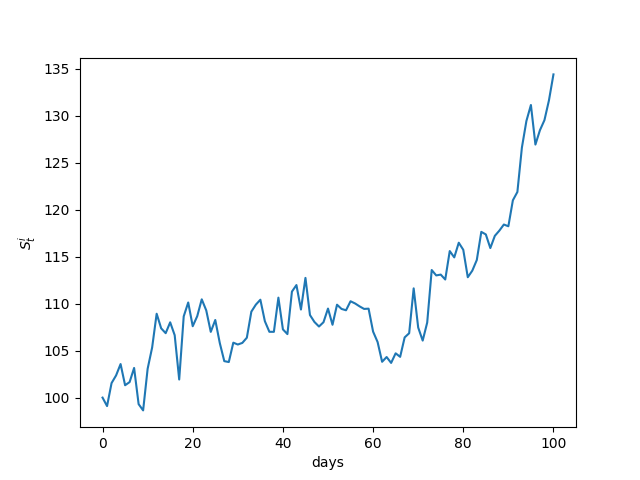
\includegraphics[width=0.5\textwidth]{figures/no_pattern}
	}
	\subfloat[Head and shoulder pattern.\label{}]{%
		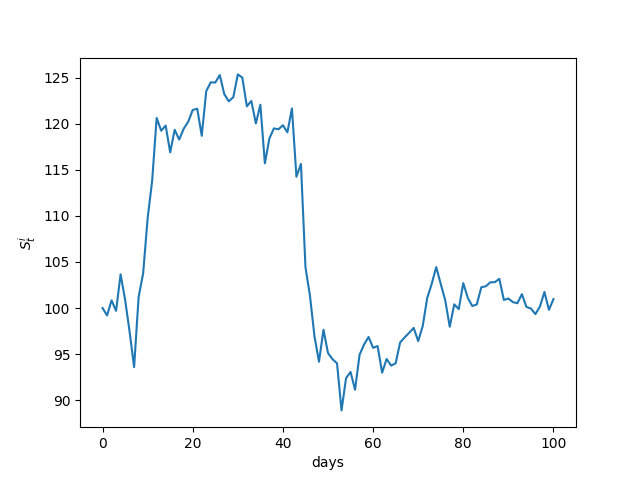
\includegraphics[width=0.5\textwidth]{figures/head_and_shoulder}
	}\\
	\subfloat[Triangle pattern.\label{}]{%
		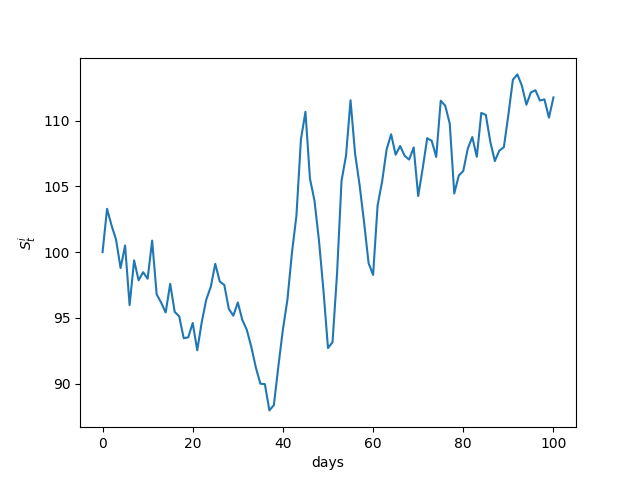
\includegraphics[width=0.5\textwidth]{figures/triangle}
	}
	\caption{Examples of time series used in the training of the CNN for technical analysis.}
	\label{fig:patterns}
\end{figure}

\begin{ipython}
import numpy as np
from finnn import FinNN

train_labels = np.load("training_techana_labels.npy")
train_images = np.load("training_techana_images.npy")
trainer = FinNN("CNN1D")
trainer.setData(train_images, train_labels)
# define the CNN
trainer.addConv1DInputLayer(filters=80, filter_size=20,
input_size=(101, 1))
trainer.addConv1DLayer(filters=80, filter_size=15)
trainer.addMaxPooling1D(3)
trainer.addConv1DLayer(filters=100, filter_size=10)
trainer.addConv1DLayer(filters=100, filter_size=5)
trainer.addGlobalAveragePooling1D()
trainer.addDropout(0.5)
trainer.addCNNOutputLayer(outputs=3)

trainer.compileModel(loss='categorical_crossentropy', opt='adam')
trainer.fit(epochs=80)
trainer.saveModel('techana')
\end{ipython}
\begin{ioutput}
Epoch 1/80
- 23s 1ms/step - loss: 0.6773
Epoch 2/80
- 23s 1ms/step - loss: 0.5421
...
Epoch 79/80
- 23s - loss: 0.0737
Epoch 80/80
- 23s - loss: 0.0692
\end{ioutput}

\begin{attention}
\subsubsection{Dropout}

Large neural nets trained on relatively small datasets can overfit the
training data.

This has the effect of the model learning the statistical noise in the
training data, which results in poor performance when the model is
evaluated on new data (e.g. a test dataset).

One approach to reduce overfitting is to fit all possible different
neural networks on the same dataset and to average the predictions from
each model. This is not feasible in practice, and can be approximated
using a small collection of different models, called an ensemble. A
problem even with the ensemble approximation is that it requires
multiple models to be fit and stored, which can be a challenge if the
models are large, requiring days or weeks to train and tune.

\emph{Dropout} is a regularization method that approximates training a
large number of neural networks with different architectures in
parallel.

During training, some number of layer outputs are randomly ignored or
\emph{dropped out}. This has the effect of making the layer look-like
and be treated-like a layer with a different number of nodes and
connectivity to the prior layer. In effect, each update to a layer
during training is performed with a different ``view'' of the configured
layer.

Even if the it may seems counter intuitive (better training when
switching off nodes) indeed dropout breaks-up situations where network
layers co-adapt to correct mistakes from prior layers, in turn making
the model more robust.
\end{attention}

The performance test is carried on in simulated real case scenario where
a time series is analyzed in real-time in order to predict as soon as
possible a particular pattern and take advantage of the prediction.

To do so it has been presented to the CNN sliding windows of a series
to simulate the flowing of the time. So if for example the time series is made
of 100 points (e.g. each point representing a hourly measurement),
it has been given in input to the CNN first the points between
\([0, 80]\), then \([0, 81]\), \([0, 82]\) and so on to simulate new real
time data incoming. 

The goal was to check when the neural network was
capable of predicting the incoming pattern. Figure~\ref{fig:frame_simulation}
shows the "temporal frames" that have been presented to the CNN.

\begin{figure}
	\centering
	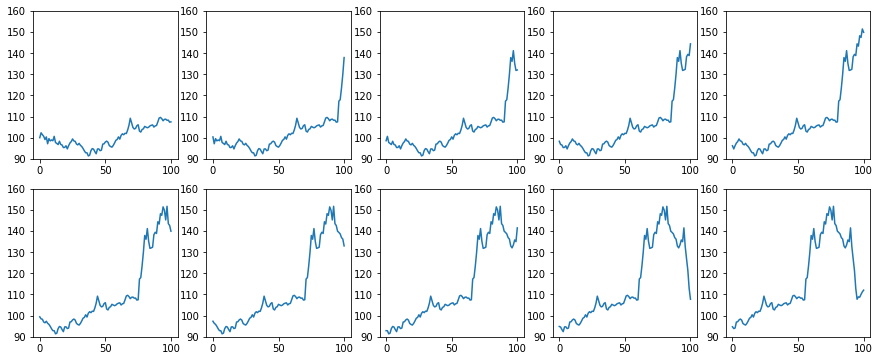
\includegraphics[width=\textwidth]{figures/tech_ana_frames.png}
	\caption{Ten frames simulating closing price date incoming in real time. The CNN was tested to check if and when it would have been able to detect any pattern in data.}
	\label{fig:frame_simulation}
\end{figure}


\begin{ipython}
test_images = np.load("testing_techana_frames.npy")
trainer.loadModel("techana")
predictions = trainer.predict(test_images)

for i in range(len(predictions)):
    print (np.argmax(predictions[i]), ["{:.3f}".format(p) for p in predictions[i]])
\end{ipython}
\begin{ioutput}
0 ['0.942', '0.000', '0.058']
0 ['0.970', '0.000', '0.030']
0 ['1.000', '0.000', '0.000']
0 ['0.999', '0.001', '0.000']
0 ['0.784', '0.216', '0.000']
1 ['0.000', '1.000', '0.000']
1 ['0.000', '1.000', '0.000']
1 ['0.000', '1.000', '0.000']
1 ['0.000', '1.000', '0.000']
1 ['0.000', '1.000', '0.000']
\end{ioutput}
\noindent
The arrays in the output represent the likelihood assigned by the CNN to the series for each category
at each time interval. So up to $t=4$ the CNN is more than 95\% sure there is no pattern. 
At $t=5$ the CNN starts to recognize a pattern assigning about 20\% probability to the "head and shoulder" class.
For $t\geq 6$ the neural network clearly recognizes the pattern.

	
\begin{thebibliography}{9}
\bibitem{bib:deep_learning} I. Goodfellow, Y. Bengio and A. Courville, \href{http://www.deeplearningbook.org}{\emph{Deep Learning}}, MIT Press, 2016
\bibitem{bib:nn_over_human}K. Grace, J. Salvatier, A. Dafoe, B. Zhang and O. Evans, \emph{When Will AI Exceed Human Performance? Evidence from AI Experts}, arXiv:1705.08807, 2005
\bibitem{bib:activation_function} J. Lederer, \emph{Activation Functions in Artificial Neural Networks: A Systematic Overview}, arxiv: 2101.09957, 2001
\bibitem{bib:backpropagation}\href{https://towardsdatascience.com/understanding-backpropagation-algorithm-7bb3aa2f95fd}{\emph{Understanding back-propagation algorithm}}, Towards Data Science [Online]
\bibitem{bib:loss_function}\href{https://medium.com/human-in-a-machine-world/mae-and-rmse-which-metric-is-better-e60ac3bde13d}{\emph{Mae and rmse which metric is better ?}}, Medium [Online]
\bibitem{bib:keras}\href{https://keras.io/}{\emph{Keras Documentation}}, [Online]  
\bibitem{bib:tensorflow}\href{https://www.tensorflow.org/}{\emph{Tensorflow Documentation}}, [Online] 
\bibitem{bib:scikit}\href{https://scikit-learn.org/stable/}{\emph{scikit-learn Documentation}}, [Online]
\end{thebibliography}